% !TeX spellcheck = pl_PL
\documentclass[a4paper]{article}
\usepackage{polski}
\usepackage[utf8]{inputenc}
\usepackage{lmodern}
\usepackage{indentfirst}
\usepackage{graphicx}
\usepackage{amsmath}
\usepackage[unicode, bookmarks=true]{hyperref} %do zakładek
\usepackage{tabto} % do tabulacji
\NumTabs{6} % globalne ustawienie wielkosci tabulacji
\usepackage{array}
\usepackage{multirow}
\usepackage{listings}
\usepackage{array}
\usepackage{dcolumn}
\usepackage{bigstrut}
\usepackage{color}
\usepackage{epigraph}
\usepackage{wrapfig}
\usepackage{MnSymbol}
\usepackage{xparse}
\usepackage[usenames,dvipsnames]{xcolor}
\usepackage[T1]{fontenc}
\usepackage{enumitem}
\usepackage{courier}
\usepackage[toc,page]{appendix}
\usepackage{listings}

\lstset{basicstyle=\footnotesize\ttfamily,breaklines=true}
\lstset{framextopmargin=50pt,frame=leftline}

%załączniki - polskie nazwy 
\renewcommand\appendixtocname{Załącznik} %spis treści 
\renewcommand\appendixpagename{Załącznik} %strona sekcji 

\makeatletter
\newcommand*{\rom}[1]{\expandafter\@slowromancap\romannumeral #1@}
\makeatother

\setlength{\epigraphwidth}{0.5\textwidth}

\newcommand{\HRule}{\rule{\linewidth}{0.5mm}}
\setlength{\textheight}{24cm}
\setlength{\textwidth}{15.92cm}
\setlength{\footskip}{10mm}
\setlength{\oddsidemargin}{0mm}
\setlength{\evensidemargin}{0mm}
\setlength{\topmargin}{0mm}
\setlength{\headsep}{10mm}
\setlength{\voffset}{-7mm}

\lstset{language=C++,
	keywordstyle=\color{blue},
	stringstyle=\color{red},
	commentstyle=\color{green},
	morecomment=[l][\color{magenta}]{\#}
}

\makeatletter
\def\@seccntformat#1{%
	\expandafter\ifx\csname c@#1\endcsname\c@section
	\thesection.
	\else
	\csname the#1\endcsname\quad
	\fi}
\makeatother

%\titlespacing*{\section}
%{0pt}{0pt}{-0.2cm}

\usepackage{fancyhdr} % Required for modifying headers and footers
\fancyhead[L]{\textsf{\rightmark}} % Top left header
\fancyhead[R]{\textsf{\leftmark}} % Top right header
\renewcommand{\headrulewidth}{1.2pt} % Rule under the header
\fancyfoot[C]{\textbf{\textsf{\thepage}}} % Bottom center footer
\renewcommand{\footrulewidth}{1.2pt} % Rule under the footer
\pagestyle{fancy} % Use the custom headers and footers throughout the document

\usepackage{titlesec}
\makeatletter
\@addtoreset{section}{part}
\makeatother

\titleformat{\paragraph}
{\normalfont\normalsize\bfseries}{\theparagraph}{1em}{}
\titlespacing*{\paragraph}
{0pt}{3.25ex plus 1ex minus .2ex}{1.5ex plus .2ex}

\begin{document}
	%\kslistofremarks
	%	\maketitle
	% !TeX spellcheck = pl_PL
\begin{titlepage}
	\begin{center}
		
		% Upper part of the page. The '~' is needed because \\
		% only works if a paragraph has started.
		
\includegraphics[width=0.5\textwidth]{logo.png}~\\[1cm]
		%?[width=0.15\textwidth]
		
		\textsc{\LARGE Politechnika Śląska w Gliwicach}\\[1.5cm]
		
		\textsc{\Large Zaawansowane Biblioteki Programistyczne}\\
		\textsc{\today}\\[0.5cm]
		
		% Title
		\HRule \\[0.4cm]
		{ \huge \bfseries Grupowanie metodą k-średnich \\[0.4cm] }
		
		\HRule \\[1.5cm]
		
		% Author and supervisor
		\textsc{\Large Autor:} \\
		Bartłomiej Buchała \\
		[1.0cm]
		Informatyka SSM, semestr II \\
		Rok akademicki 2016/2017 \\
		Grupa OS1
		
		\vfill

	\vfill
\end{center}
\end{titlepage}
	
	\tableofcontents
	\newpage
		
	\input{intro.tex}
	
	\section{Analiza problemu}

Przed przystąpieniem do pracy nad algorytmem, należało rozwiązać kilka problemów projektowych.

\subsection{Problem doboru punktów początkowych}

Podstawowym krokiem przy każdym wywołaniu algorytmu jest ustalenie punktów początkowych. Wyniki algorytmu k-średnich silnie zależą od wyboru punktów początkowych, jednak nie ma ściśle określonej reguły, jak je należy wybierać. W zależności od startowej wartości centroidów, wyniki grupowania mogą być inne z każdym uruchomieniem algorytmu (nawet przy identycznych parametrach). Początkowo wydaje się, że wybór losowych współrzędnych jest dobrym rozwiązaniem. Przeszkodą jest jednak założenia generyczności algorytmy -- istnieje możliwość wyboru losowego punktu pośród wartości typu int lub klasy reprezentującej punkt na płaszczyźnie dwuwymiarowej, jednak zadanie jest znacznie utrudnione w przypadku np. typu string lub klasy zewnętrznej pochodzącej z innego projektu. W takim przypadku warunkiem uniemożliwiającym wybór losowych współrzędnych jest brak wiedzy na temat budowy typu lub nawet niemożliwość utworzenia obiektu o losowych współrzędnych.

Rozwiązaniem problemu jest wybór losowych elementów z zakresu podanego do grupowania. W pierwszej iteracji środki skupień znajdują się dokładnie w tym samym miejscu, w którym istnieją niektóre z danych wejściowych.

\subsection{Miara odległości}\label{metric}

Algorytm ma zapewniać generyczność -- dlatego dla typu danych na którym chcemy wykonać grupowanie musi istnieć miara odległości (metryka), pozwalająca określić odległość pomiędzy dwoma dowolnymi elementami tego typu (w najczęstszym scenariuszu - pomiędzy daną wejściową, a centroidem). Zakłada się, że odległość ewaluowana jest jako wartość typu \texttt{double}. W celu zapewnienia poprawności działania algorytmu, konieczne jest przekazanie do funkcji grupującej obiektu funkcyjnego (z przeciążonym operatorem \texttt{()}) zwracającą wartość zmiennoprzecinkową, będącą miarą odległości pomiędzy 2 elentami. Przykład implementacji dla typy \texttt{int} znajduje się poniżej.

\begin{lstlisting}
/// <summary>
/// Obiekt funkcyjny, bedacy miara odleglosci pomiedzy dwoma wartosciami typu int.
/// </summary>
struct Int_distance
{
	inline double operator()(int p1, int p2)
	{
		return (double)abs(p1 - p2);
	}
};
\end{lstlisting}

Sposób w jaki implementowana jest metryka leży w pełni w kwestii osoby korzystającej z algorytmu. Dla punktów w przestrzeni dwuwymiarowej może to być metryka euklidesowa lub miejska (Manhattan), dla typu char odległość dzieląca znaki w tablicy ASCII, itp.

\subsection{Funkcja uśredniejąca}\label{avg}

Podobnie jak w przypadku metryki, z powodu generyczności funkcji konieczne jest zadeklarowanie obiektu funkcyjnego określającego, w jaki sposób obliczany będzie nowy centroid spośród n elementów należących do skupienia. Funktor powinien pozwalać na 2 operacje:

\begin{itemize}
	\item Kumulację obiektów -- dodanie nowego obiektu (przekazanego jako referencję) do skumulowanej wartości oraz inkrementacja licznika dodanych punktów. Realizowane przez przeciążony operator \texttt{+=}.
	\item Uśrednienie -- wyliczenie nowych współrzędnych centroidu na podstawie skumulowanej wartości oraz liczby skumulowanych elementów. Realizowane przez przeciążony operator \texttt{()}. Jako parametr należy przekazać obiekt obliczanego typu -- jest to poprzednia wartość środku skupienia. Jeżeli liczba obiektów należących do danej grupy jest większa niż 0, przekazany obiekt jest aktualizowany do wartości nowego centroidu. Jeżeli liczba elementów w grupie jest równa 0, centroid nie jest nadpisywany
\end{itemize}

Przykład implementacji uśredniającego obiektu funkcyjnego dla typi \texttt{int} znajduje się poniżej.

\begin{lstlisting}
struct Int_average
{
	/// Wartosc domyslna nowego centroidu.
	int newCentroid = 0;
	
	/// Licznik kumulowanych wartosci.
	int count = 0;
	
	/// <summary>
	/// Przeciazony operator (), wyliczajacy nowa wartosc centroidu usredniona z n elementow.
	/// </summary>
	/// <param name="oldCentroid">Aktualna wartosc centroidu</param>
	inline void operator()(int &oldCentroid)
	{
		if (count != 0)
			newCentroid = (int)(newCentroid / count);
		else
			newCentroid = oldCentroid;
		
		oldCentroid = newCentroid;
		
		newCentroid = 0;
		count = 0;
	}
	
	/// <summary>
	/// Przeciazony operator +=, kumulujacy kolejna wartosc.
	/// </summary>
	/// <param name="value">Kolejna kumulowana wartosc.</param>
	inline void operator +=(const int & value)
	{
		newCentroid += value;
		
		count++;
	}
};
\end{lstlisting}

Warunkiem koniecznym do poprawnego działania algorytmu jest zadeklarowanie obiektu funkcyjnego z przeciążonymi operatorami () oraz += przyjmującymi po jednym parametrze typu tożsamego do grupowanych danych. Reszta szczegółów dotyczących implementacji leży w kwestii użytkownika.

\subsection{Warunki stopu}\label{stop}

Zaimplementowana funkcja pozwala na wybór jednego z dwóch (lub obu jednocześnie) warunku zatrzymania wykonywania algorytmu.

\begin{itemize}
	\item Maksymalna liczba iteracji -- program kończy grupowanie elementów po wykonaniu określonej liczby iteracji zadanej jako parametr wejściowy.
	\item Osiągnięcie stanu stabilnego -- jako stan stailny określamy sytuację, w której w dwóch kolejnych iteracjach nie nastąpi żadna zmiana przynależności do skupienia.
\end{itemize}

Podanie warunku stopu jako parametr odbywa się przez typ wyliczeniowy.
	
	\section{Specyfikacja zewnętrzna}

\subsection{Wykorzystanie algorytmu}

Program został przygotowany zgodnie z myślą wykorzystania podobną do algorytmu sortowania znajdującego się w standardowej bibliotece wzorców (\texttt{std::sort()}). Wykorzystanie algorytmu odbywa się w kilku krokach:

\begin{enumerate}
	\item Dołączenie pliku nagłówkowego do projektu poprzez zastosowanie komendy:
	
	\begin{lstlisting}
#include "K_means.h"
	\end{lstlisting}
	
	\item Utworzenie elementu klasy szablonowej o konkretnym typie:
	
	\begin{lstlisting}
K_means<Typ_Danych> k_means;
	\end{lstlisting}

	Gdzie <Typ\textunderscore Danych> oznacza dowolny, dostarczony przez użytkownika typ danych.
	
	\item Wykonanie algorytmu grupowania k-średnich
	\begin{lstlisting}	
result = k_means.Group(first, last, distanceMeasure, groupAverage, k, MaxIterations, StopCondition, PrintOutput);
	\end{lstlisting}
	
	Elementem zwróconym będzie wektor iteratorów wskazujących na pierwsze elementy grup posortowanych elementów.
	
	\item Opcjonalnym krokiem jest wywołanie wyświetlenia elementów kolekcji za pomocą funkcji DisplayCollection. Aby funkcja działała poprawnie, elementy w zakresie muszą implementować operator <<.
	\begin{lstlisting}	
DisplayCollection(Iterator first, Iterator last)
	\end{lstlisting}
\end{enumerate}

\subsection{Opis parametrów wywołania funkcji Group}

\begin{description}
	\item[first] -- jest iteratorem swobodnego dostępu (używanym w takich strukturach jak na przykład vector czy deque ze standardowej biblioteki wzorców) wskazującym na pierwszy element z grupowanego zakresu.
	\item[last] -- jest iteratorem swobodnego dostępu (używanym w takich strukturach jak na przykład vector czy deque ze standardowej biblioteki wzorców) wskazującym na ostatni element z grupowanego zakresu.
	\item[distanceMeasure] -- obiekt funkcyjny opisujący metrykę pomiędzy elementami danego typu. Więcej informacji można znaleźć w podrozdziale \ref{metric}.
	\item[groupAverage] -- obiekt funkcyjny opisujący funkcję uśredniającą elementy danego typu. Więcej informacji można znaleźć w podrozdziale \ref{avg}.
	\item[k] -- określa maksymalną liczbę iteracji algorytmu. W przypadku, gdy parametr \texttt{StopCondition} ustawiony jest na \texttt{StableState}, wartość tego parametru jest nieistotna.
	\item[StopCondition] -- określa warunek stopu (\ref{stop}). Jest to argument typu wyliczeniowego i przyjmuje jedną z 3 wartości:
	\begin{itemize}
		\item MaxIterations -- warunkiem stopu jest wykonanie odpowiedniej liczby iteracji (podanej w parametrze \texttt{k}).
		\item StableState -- program wykonuje się tak długo, aż w kolejnych iteracjach nie nastąpi zmiana przynależności do skupienia żadnego pośród wszystkich grupowanych elementów.
		\item Both -- połączenie powyższych. Program wykonuje się identycznie jak w przypadku \texttt{StableState}, jednak może się zakończyć wcześniej jeżeli została wykonana określona liczba iteracji
	\end{itemize}
	\item[PrintOutput] -- określa, czy informacje o współrzędnych centroidów i przynależności punktów do skupień mają być wypisywane na strumień wyjściowy. Uwaga: może znacznie zwiększyć czas wykonywania algorytmu.
\end{description}

Przykładowe wywołanie funkcji dla wektora o elementach typu całkowitego:

	\begin{lstlisting}	
result = k_means.Group(vec.begin(), vec.end(), Point2D_distance(), Point2D_average(), 4, 3, StableState, false);
	\end{lstlisting}

Gdzie \texttt{vec} jest wektorem ze standardowej biblioteki wzorców zawierającym wartości typu \texttt{int}, a \texttt{Point2D\textunderscore distance()} i \texttt{Point2D\textunderscore average()} są obiektami funkcyjnymi stworzonymi zgodnie z zasadami opisanymi w podrozdziałach \ref{metric} i \ref{avg}.

\subsection{Opis parametrów wywołania funkcji DisplayCollection}

\begin{description}
	\item[first] -- jest iteratorem swobodnego dostępu (używanym w takich strukturach jak na przykład vector czy deque ze standardowej biblioteki wzorców) wskazującym na pierwszy element z grupowanego zakresu.
	\item[last] -- jest iteratorem swobodnego dostępu (używanym w takich strukturach jak na przykład vector czy deque ze standardowej biblioteki wzorców) wskazującym na ostatni element z grupowanego zakresu.
\end{description}

Przykładowe wywołanie funkcji dla wektora o elementach typu całkowitego:

\begin{lstlisting}	
k_means.DisplayCollection(vec.begin(), vec.end());
\end{lstlisting}

Gdzie \texttt{vec} jest wektorem ze standardowej biblioteki wzorców zawierającym wartości typu \texttt{int}.

\subsection{Przykład scenariusza użycia}

Dla poniższego kodu:

\begin{lstlisting}	
	K_means<Point_2D> k_means;
	vector<Point_2D> vec = vector<Point_2D>();
	
	//Fill vec with data
	
	k_means.DisplayCollection(vec.begin(), vec.end());
	
	auto result = k_means.Group(vec.begin(), vec.end(), Point2D_distance(), Point2D_average(), 3, 2, StableState, true);
	
	k_means.DisplayCollection(vec.begin(), vec.end());
\end{lstlisting}

Wynik działania będzie następujący:

\begin{figure}[h]
	\centering
	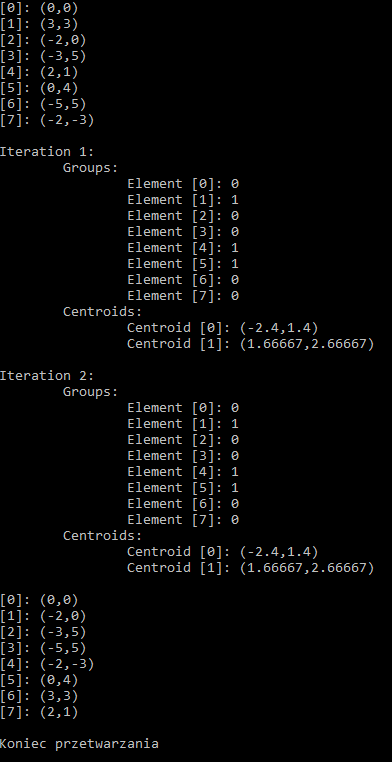
\includegraphics[width=0.35\textwidth]{./img/example.png}
	\caption{Przykładowe wywołanie algorytmu}
	\label{img:example}
\end{figure}
	
	\section{Specyfikacja wewnętrzna}

\subsection{Struktura projektu}

Solucja aplikacji zawiera 6 plików. Większość deklaracji funkcji znajduje się w plikach nagłówkowych -- ze względu na generyczność klasy niemożliwa jest deklaracja fragmentów kodu w plikach źródłowych. Kompilator tworzy klasy szablonowe na etapie kompilacji.

\begin{description}
	\item[main.cpp] jest plikiem poglądowym i zawiera scenariusze testowe wykorzystania algorytmu. Nie stanowi integralnej części reszty projektu i służy jedynie pokazaniu przykładowych użyć algorytmu.
	\item[bitmap\textunderscore image.hpp] -- plik biblioteki zewnętrznej pochodzący ze strony \url{http://www.partow.net/programming/bitmap/index.html}. Dzięki funkcjom zadeklarowanym w tym pliku możliwe jest wczytywanie bitmap do aplikacji napisanej w języku C++ i ich modyfikacja/zapis. Fragmenty tej biblioteki wykorzystywane są w pliku \texttt{main.cpp} do testowania algorytmu na bitmapach.
	\item[IntTest.h] -- plik zawierający obiekty funkcyjne metryki i funkcji uśredniającej dla liczb całkowitych.
	\item[Point\textunderscore 2D.h] -- zawiera deklaracje następujących elementów:
	\begin{itemize}
		\item Klasa \textbf{Point\textunderscore 2D} -- klasa reprezentująca punkt na płaszczyźnie euklidesowej. Posiada 2 pola zmiennoprzecinkowe (x i y), odpowiadająca odpowiednio współrzędnym na osiach x i y.
		\item Przeciążony \textbf{operator <<} dla typu Point\textunderscore 2D -- pozwala na wypisanie wyżej wymienionej klasy na strumień wyjściowy.
		\item Obiekt funkcyjny \textbf{Point2D\textunderscore distance} -- funktor określający w jaki sposób ma zostać obliczona odległość pomiędzy dwoma obiektami klasy Point\textunderscore 2D.
		\item Obiekt funkcyjny \textbf{Point2D\textunderscore average} -- funktor określający w jaki sposób kumulować oraz uśrednić wartość z wielu obiektów typu Point\textunderscore 2D.
	\end{itemize}
	\item[K\textunderscore means.h] -- plik zawierający główną klasę K\textunderscore means szerzej opisaną w punkcie \ref{kmeans}.
\end{description}

\subsection{Klasa K\textunderscore means}\label{kmeans}

\subsubsection{Typy}

\begin{description}
	\item[returnIterator] -- jest typem zwracanym prze funkcję \texttt{Group}. W rzeczywistości jest to iterator wektora, którego elementy wskazują na wartości typu zdefiniowanego przez użytkownika (elementy wejściowe).
\end{description}

\subsubsection{Pola}

\begin{description}
	\item[Centroids] -- współrzędne centroidów (środków grup). Zmieniają się co iterację.
	\item[currentGroupId] -- tablica wartości całkowitych przechowująca informację o aktualnej przynależności danych do grup. Wartość i-tej komórki odpowiada numerowi grupy do której należy i-ty element.
	\item[nextGroupId] -- tablica wartości całkowitych przechowująca informację o przynależności danych do grup w następnej iteracji. Wartość i-tej komórki odpowiada numerowi grupy do której będzie należeć i-ty element.
	\item[distancesMatrix] -- macierz wartości zmiennoprzecinkowych określająca odległość danych od środków grup. Indeks kolumny odpowiada numerowi grupy, a indeks wiersza numerowi elementu.
	\item[returnValues] --  wektor iteratorów typu \texttt{returnIterator} wskazujących na elementy będące kolejnymi początkami grup.
	\item[iterationCounter] -- licznik iteracji algorytmu, służy do sprawdzania warunku stopu.
	\item[groupNumber] -- liczba grup (skupień) podanych przez użytkownika.
	\item[elementCount] -- liczba elementów znajdujących się w zakresie określonym iteratorami początku i końca. Wyliczana na podstawie argumentów przekazywanych przez użytkownika.
	\item[stopConditionFulfilled] -- flaga określająca, czy został spełniony warunek stopu. Sprawdzana na końcu każdej iteracji.
	\item[groupMinimum] -- zmienna pomocnicza przechowująca informację o najmniejszej odległości punktu pośród wszystkich odległości pomiędzy punktem a centroidami.
	\item[groupStartIndex] -- zmienna pomocnicza używana w trakcie obliczania indeksu elementu wskazywanego przez iterator początku grupy.
	
\end{description}

\subsubsection{Metody}

\begin{description}
	\item[void DisplayCollection(Iterator first, Iterator last)]  -- metoda nie integrujaca się z głównym algorytmem. Jej zadaniem jest wyświetlenie wszystkich elementów kolejkcji począwszy od elmentu wskazywanego przez iterator \texttt{first}, a kończąc na elemencie wskazywanym przez iterator \texttt{last}. Typ danych musi posiadać przeciążony operator \texttt{<<}.
	\begin{itemize}
		\item \texttt{Iterator first} -- iterator wskazujący na element typu podanego przez użytkownika będącym początkiem zakresu.
		\item \texttt{Iterator last} -- iterator wskazujący na element typu podanego przez użytkownika będącym końcem zakresu.
	\end{itemize}
	
	\item \textbf{returnIterator* Group(Iterator first, Iterator last, DistancePredicate \&distanceMeasure, AveragePredicate \&groupAverage, int maxIteration, int k, StopConditions stopCondition, bool printOutput = false)} -- dyspozytor iteratora swobodnego dostępu. Stanowi zabezpiecznie przed użyciem funkcji dla innych typów iteratorów. Parametry wywołania są tożsame z funkcją właściwą (za wyjątkiem znacznika iteratora) i opisane są w punkcie \ref{parameters}.
	
	\item \textbf{returnIterator* Group(Iterator first, Iterator last, std::random\textunderscore access\textunderscore iterator\textunderscore tag, DistancePredicate \&distanceMeasure, AveragePredicate \&groupAverage, int maxIteration, int k, StopConditions stopCondition, bool printOutput)} -- główna funkcja implementująca algorytm grupowania metodą k-średnich. Znaczenie parametrów wywołujących opisane jest w punkcie \ref{parameters}. \texttt{std::random\textunderscore access\textunderscore iterator\textunderscore tag} jest parametrem dodawanym sztucznie przez funkcję dyspozytora -- ponieważ publicznie dostępnie jest jedynie dyspozytor, uniemożliwia to podanie argumentów iteratora nie będącymi iteratorami swobodnego dostępu. Jest to sposób wykorzystywany w standardowej bibliotece wzorców przy funkcji \texttt{std::distance()}. W ciele funkcji wywoływana jest funkcja zgodnie z założeniami algorytmu (\ref{algorithm}).
	
	\item[void Initialize()] -- funkcja wywoływana na samym początku funkcji \texttt{Group}. Zajmuje się sprawdzeniem poprawności argumentów (ilość grup, zakres elementów), zaalokowaniem pamięci na struktury pomocnicze (\texttt{Centroids}, \texttt{returnValues}, \texttt{currentGroupId}, \texttt{nextGroupId} oraz \texttt{distancesMatrix}) w zależności od ilości skupień oraz elementów do pogrupowania. Ustawia również pola na odpowiednie wartości w celu przygotowania do nowego wykonania algorytmu (ustawienie \texttt{iterationCounter} oraz \texttt{groupStartIndex} na 0, \texttt{stopConditionFulfilled} na \texttt{false} oraz \texttt{groupMinimum} na \texttt{DBL\textunderscore MAX} odpowiadającej maksymalnej wartości zmiennoprzecinkowej).
	
	\item[void AssignStartingPoints(Iterator first)] -- funkcja wywoływana w funkcji \texttt{Group} zaraz po funkcji \texttt{Initialize}. Spośród wszystkich elementów wejściowych wybiera \texttt{groupNumber} początkowych wartości centroidów. Jako argument funkcja \texttt{Group} przekazuje do niej iterator wskazujący na pierwszy element.
	
	\item[void DisplayCurrentIterationState()] -- metoda wyświetlająca informacje o aktualnej przynależności danych do grup oraz współrzędnych centroidów. Jest ona wywoływana przy każdej iteracji algorytmu, o ile parametr \texttt{printOutput} ustawiony został na wartość \texttt{true}.
	
	\item[void Finish()] -- metoda wywoływana pod koniec metody \texttt{Group} dealokująca pamięć struktur tymczasowych inicjalizowanych w metodzie \texttt{Initialize} -- jedynym wyjątkiem jest struktura \texttt{returnValues}, która jest zwracana poza klasę.
\end{description}
	
	\section{Testowanie aplikacji}
	
	\section{Podsumowanie}

\end{document}


